%
% main.tex -- Paper zum Thema thermohaline
%
% (c) 2018 Jonas Gründler, Hochschule Rapperswil
%
\chapter{3-Box-Modell der Thermohalinen Zirkulation\label{chapter:thermohalin}}
\lhead{3-Box-Modell der Thermohalinen Zirkulation}
\begin{refsection}
\chapterauthor{Jonas Gründler}

%% Structure:
% Einleitung (Beschreibung schon in Teil Mueller)
%		-Thermohaline Zirkulation, was ist das
%		-Einfluss Temperatur, Salz
%		-Darstellung und Erklärung mittels Bildern (Erste Dichte-Gleichung)
%		-
%		-ev. Vertiefung der Mechanismen
%		-Beschreibung der Erweiterung und Einschränkungen der Simulation.
%		-Allgemein Einschränkung von simulationen
%		-Erhöhung der komplexizität bei erhöhung der Boxzahl
%		-
%
% Hauptteil
% 		-Erweiterung des Modells auf 3 Boxen (4 Boxen)
% 		-Getroffene Annahmen und Vereinfachungen
%		-Golfrstrom und Auswirkungen der THC
% 		-Annahme der Umdrehung oder des Stillstandes, mit Auswirkungen
% 
%

%Notes
% -Windeinfluss (gross auf golfstrom)
% -Sverdrup (one million cubic meters per second)
% -Wasserschichten (mixing layer, thermocline region, abyssal zone)
% -Sea temperature as function of z(depth), p.32 (diff equation and solution)
% -Picture water structure
	\section{THC, Was ist das?}
\rhead{THC, Was ist das?}

Die "THC", ausgeschrieben thermohaline Zirkulation. Ist eine Weltumspannende Meeresströmung welche in verschiedene Abschnitte aufgeteilt werden kann.
Diese Strömungen sorgen für eine Durchmischung der verschiedenen Ozeane. So erzeugen sie einen Wärme- und Nährstoffaustausch in den verschiedenen Weltregionen. 
Die Auswirkung dieses Energieaustausches sind spürbar, so heizt zum Beispiel der Golfstrom, welcher Auch zu diesen Strömungen gehört Nordeuropa um mehrere Grad auf.
Doch wie entsteht diese Strömung?
Hier spielen viele Einflüsse eine Rolle. Die Verteilung der Kontinente, die Corioliskraft, die Wasserdichte und auch Wetter und Winde. 
Im Rahmen dieser Arbeit werde ich nur auf die Wasserdichte als Einfluss eingehen. Sie ist gut zu simulieren und ist durch die einfache Veränderbarkeit auch am Spannendsten.
die Verteilung der Kontinente und auch die Corioliskraft sind durch ihre kaum vorhandene Änderung als Konstanten zu betrachten. Das Letzte was noch bleibt, sind Wind und Wetter. 
Diese Einflüsse sind praktisch nicht vorherzusagen und auch ihr Einfluss variiert stark. Aus diesem Grund werden auch diese nicht Simuliert. 
Zusätzlich würde das Einbeziehen dieser grössen die Komplexität der Simulation Stark erhöhen.

\subsection{Dichte}
\rhead{Dichte}

Die Thermohaline Zirkulaton wird hauptsächlich durch Dichteunterschiede im Wasser hervorgerufen.
Dichtes Wasser sinkt ab und weniger dichtes Wasser steigt bekanntlich auf. Die Hauptsächlichen Einflussfaktoren der Wasserdichte sind:

\begin{itemize}
	\item Salzgehalt
	\item Temperatur
\end{itemize}

Durch einen hohen Salzgehalt wird das Wasser dichter. Die Temperatur hat den inversen Einfluss. Je wärmer das Wasser wird, desto weniger dicht ist es. 
Hier zwei Grafiken zur Veranschaulichung:
\begin{figure}
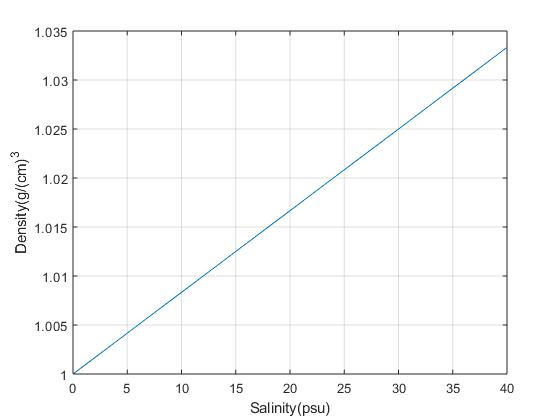
\includegraphics{code/graphs/graph_salinity.jpg}
\caption{Dichteveränderung abhängig vom Salzgehalt}
\end{figure}

\begin{figure}
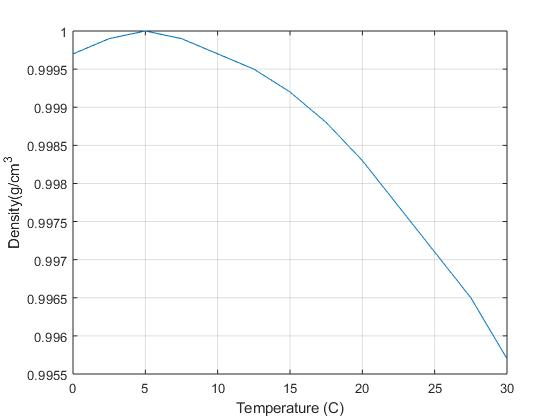
\includegraphics{code/graphs/graph_temp.jpg}
\caption{Dichteveränderung abhängig von der Temperatur}
\end{figure}

Diese Einflüsse Lassen sich in einer Gleichung zusammenfassen, welche im Hauptteil des Buches im Kapitel \ref{Salinität und Dichte} schon Besprochen wurde.

\begin{equation}
\varrho
=
\varrho_0(1-\alpha(T-T_0)+\beta(S-S_0))
\label{skript:salinity-linear}
\end{equation} 

Mittels dieser Gleichung lässt sich nun ein Simulation erstellen, mit welcher sich solche Strömungen simulieren lassen.

\subsection{Golfstrom}
\rhead{Golfstrom}

Im Rahmen dieser Arbeit habe ich versucht den Golfstrom, welcher Europa direkt beeinflusst, zu Simulieren.
Als fokussieren ich hier nur auf einen kleinen Teil der Globalen Thermohalinen Zirkulation.


\begin{figure}
	\includegraphics[]{bilder/deep_ocean_currents.jpg}
\end{figure}

Die Frage ist nun, was passiert mit dem Golfstrom, wenn Klimaerwärmung und Umweltverschmutzung weiter ansteigen?

\subsubsection{Funktionsweise}

Doch zuerst dazu, wie der Golfstrom funktioniert.
Der Golfstrom entspringt im Golf von Mexiko. Von dort aus wird das Warme Wasser von Winden und der Erdrotation nach Norden getrieben.
Auf diesem Weg kühlt das Wasser langsam ab, und wird durch die fortlaufende Verdunstung von Wasser immer salziger. Da der Einfluss der Salinität grösser ist als der der Temperatur, beginnt das Wasser im Norden, durch die nun Hohe Dichte abzusinken. Wenn das Wasser dann abgesunken ist, treibt es dem Grund des Meeres entlang bis nach Afrika, was den Kreislauf schliesst.
Wo hat der Klimawandel nun seinen Einfluss?
Um diese Frage zu beantworten, müssen wir weiter zurückschauen, genauer gesagt zum Kap der guten Hoffnungen. Denn eigentlich beginnt die Strömung schon dort. 
Dort Stellt sich die Frage, in welcher Richtung der Indische Ozean und der Atlantik ihr Salz austauschen. 
Denn eine Veränderung der Salzbilanz könnte im Norden, also vor der Küste Grönlands für eine Störung des Absinkens sorgen, und so den Strom zum erliegen bringen. 
Eine Störung der Salzzufuhr könnte also den Golfstrom zum erliegen bringen.
Hier gehen die Meinungen der Forscher jedoch auseinander. Salzmessungen im offenen Meer sind sehr schwierig. 
Im Moment zeigen diese jedoch, dass der Golfstrom weiter Salz in den Atlantik importiert und sich so selber am leben erhält.

Weiter kommt da noch die Erhöhung des CO2-Gehaltes in der Luft und die somit einhergehende Klimaerwärmung. sie hat zwei direkte Auswirkungen auf den Golfstrom:

\begin{itemize}
	\item Durch die Erhöhung der Lufttemperatur kann das Wasser auf dem Weg in den Norden nicht mehr genug abkühlen, um danach abzusinken.
	\item Das Abschmelzen der Polkappen, welches viel Frischwasser freisetzt, kann die Salzkonzentration so weit verringern, dass das Wasser, aufgrund der reduzierten Dichte, nicht mehr absinken kann.
\end{itemize}

Diese Beiden Prozesse, wären alleine in der Lage den Golfstrom zu stören, doch zusammen ist die Wirkung noch viel schlimmer.

Laut einer Studie des Forschers Liu Wei von der Universität Yale vom 04 Jan 2017 könnte dieses Szenario in den nächsten 300 Jahren tatsächlich eintreten. Sie zeigen auf, dass falls sich die Rate seit 1990 verdoppelt, der Golfstrom in den nächsten 300 Jahren versiegen könnte.

\subsubsection{Folgen}

Was passiert, falls der Golfstrom zum erliegen kommt, oder sogar seine Richtung ändert.
Ich denke der Film "The day after tomorrow" von Roman Emmerich ist bekannt. Er zeigt was passieren könnte, falls der Golfstrom zum erliegen kommt. 
Im Film versinkt innert weniger Tage die ganze Welt in einer neuen Eiszeit un alles endet im Chaos. 
Das ist natürlich ein wenig übertrieben Dargestellt, doch die Richtung stimmt. Falls der Golfstrom stoppt, würde trotz Klimaerwärmung Nordeuropa um einige Grad kälter werden.













	
	
	
	
	
	
	
	
	
	
	
	
	
\end
	
	\section{Simulation}
\rhead{Simulation}

Der erste schritt ist die Erstellung eines Modells.
Dazu wird der Golfstrom in drei Zonen aufgeteilt. Die jeweiligen Polarregionen und der Äquator werden je zu einer Zone. Diese Zonen werden dann je einer Box zugeordnet. Diese Boxen werden mittels Kanälen verbunden um so den Strom zu modellieren. 
Im laufe des Seminars wurden zwei Modelle erstellt. Der erste Ansatz (siehe \ref{thermohalin:3b2f_title}) war sehr lehrreich hatte aber schlussendlich nichts mit dem realen Golfstrom gemeinsam. Der zweite Ansatz (siehe \ref{thermohalin:3b1f_title}) war erfolgreicher und der Golfstrom kann mit diesem Modell qualitativ simuliert werden.
In den folgenden zwei Kapiteln werden diese zwei Modelle vorgestellt und die jeweiligen Resultate diskutiert.

\subsection{Zwei-Fluss Modell( 1. Ansatz)}\label{thermohalin:3b2f_title}

In diesem Modell werden die drei Boxen jeweils durch Rohre verbunden. Nun werden zwei Flüsse simuliert, die von den jeweiligen Dichtegradienten der unterschiedlichen Boxen abhängen. $q_1$ ist nur vom Dichteunterschied zwischen Box $1$ und Box $2$ abhängig. Dementsprechend hängt $q_2$ nur vom Dichteunterschied der Boxen $2$ und $3$ ab.
Der Vorteil dieser Aufteilung der Flüsse ist, dass wir sie entkoppeln können und sie nicht von der jeweiligen dritten Box abhängig sind.
Eine Darstellung des Modelles ist in Abbildung \ref{thermohalin:3b2f} zu finden.

\begin{figure}
	\centering
	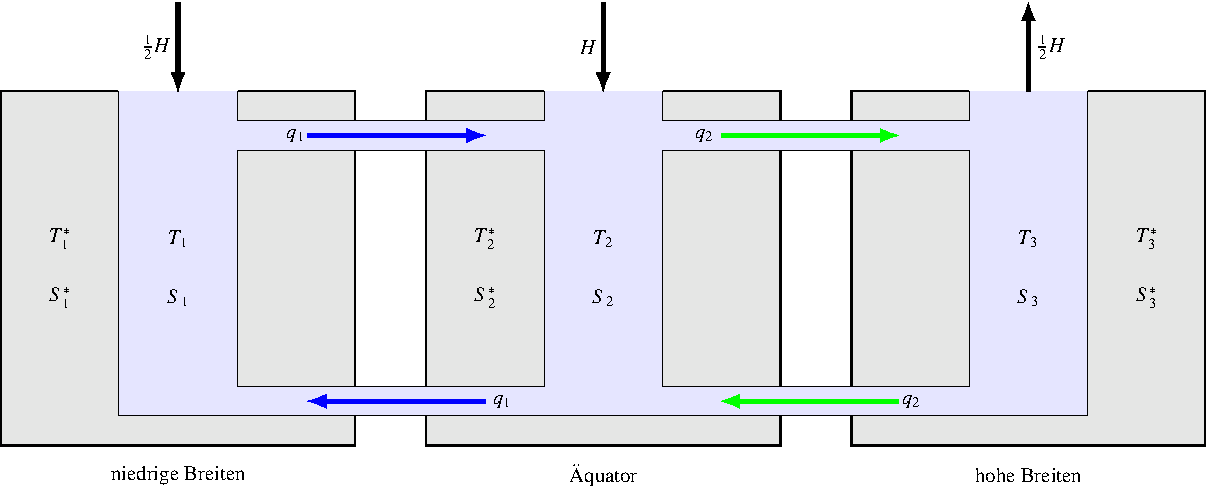
\includegraphics[width=14cm]{thermohalin/tikz/3b2f.pdf}
	\caption{Zwei-Fluss Modell des THC}
		\label{thermohalin:3b2f}
\end{figure}

Aufgrund der Darstellung lassen sich für jede Box die zugehörigen Salinitäts- und Temperaturgleichungen aufstellen. Box $1$ und $3$ haben jeweils einen Fluss in der Gleichung. Im Gegensatz dazu wird Box jedoch $3$ von zwei Flüssen durchflossen. Daraus entstehen die Gleichungssysteme \ref{thermohalin:diffgl_3b2f_temp} und \ref{thermohalin:diffgl_3b2f_salinity}. 

\begin{equation}\label{thermohalin:diffgl_3b2f_temp}
\begin{aligned}
\frac{dT_1}{dt} &= c(T_1^*-T_1)&+|q_1|(T_2-T_1)\phantom{+|q_2|(T_3-T_2)}
\\
\frac{dT_2}{dt} &= c(T_2^*-T_2)&+|q_1|(T_1-T_2)+|q_2|(T_3-T_2)
\\
\frac{dT_3}{dt} &= c(T_3^*-T_3)&+ \phantom{+|q_1|(T_1-T_2)}|q_2|(T_2-T_3)
\end{aligned}
\end{equation}
\begin{equation}\label{thermohalin:diffgl_3b2f_salinity}
\begin{aligned}
\frac{dS_1}{dt} &= -\frac{H}{2} &+ d(S_1^*-S_1)&+|q_1|(S_2-S_1)\phantom{+|q_2|(S_3-S_2)}
\\
\frac{dS_2}{dt} &= \phantom{-}H &+ d(S_2^*-S_2)&+|q_1|(S_1-S_2)+|q_2|(S_3-S_2)	
\\
\frac{dS_3}{dt} &= -\frac{H}{2} &+d(S_3^*-S_3)&+ \phantom{+|q_1|(S_1-S_2)}|q_2|(S_2-S_3)
\end{aligned}
\end{equation}	

Der erste Term auf der rechten Seite

\begin{equation*}
	c(T_i^*-T_i), \quad d(S_i^*-S_i)
\end{equation*}

stellt jeweils den Energie- und Salzaustausch mit dem umgebenden Reservoir dar. Als die Übertragungskonstante multipliziert mit der Temperaturdifferenz zwischen Box und Reservoir. Die anderen Terme auf der rechten Seite sind die Flüsse

\begin{equation*}
	|q_x|(T_i-T_j)
\end{equation*}

 welche mit der Temperaturdifferenz der jeweiligen Boxen multipliziert werden um die Effizienz der Übertragung zwischen den Boxen zu berechnen.  


Die stärke des Flusses wird aus dem Dichteunterschied zwischen den jeweiligen Boxen berechnet. 
Die Gleichungen für die Flüsse $q_x$ sind also 
\begin{equation}
\begin{aligned}
	q_1 &= k\frac{\varrho_1-\varrho_2}{\varrho_0}
	\\
	q_2 &= k\frac{\varrho_2-\varrho_3}{\varrho_0}
\end{aligned}.
\end{equation}

Für $\varrho_i$ wird dann jeweils die Formel \ref{thermohalin:Dichte} eingesetzt um die Dichte aus den jeweiligen Salinitäten und Temperaturen zu berechnen. Daraus folgt

\begin{equation}
\begin{aligned}
q_1 &= k\frac{\varrho_0[1-\alpha(T_1-T_0)+\beta(S_1-S_0)]-\varrho_0[1-\alpha(T_2-T_0)+\beta(S_2-S_0)]}{\varrho_0}
\\
q_2 &= k\frac{\varrho_0[1-\alpha(T_2-T_0)+\beta(S_2-S_0)]-\varrho_0[1-\alpha(T_3-T_0)+\beta(S_3-S_0)]}{\varrho_0}.
\end{aligned}
\end{equation}

Die Faktoren $\varrho_0, T_0$ und $S_0$ lassen sich kürzen, sodass am Schluss folgende Flussgleichungen entstehen.

\begin{equation}
\begin{aligned}
 q_1 &= k[\alpha(T_2-T_1)-\beta(S_2-S_1)] 
 \\
 q_2 &= k[\alpha(T_3-T_2)-\beta(S_3-S_2)]
\end{aligned}
\end{equation}

Da die Flüsse nur von den Differenzen der jeweiligen Boxen abhängig sind, kann man sie auch so schreiben:

\begin{equation}
\begin{aligned}
q_1 &= k[\alpha(\Delta T_{q1})-\beta(\Delta S_{q1})] 
\\
q_2 &= k[\alpha(\Delta T_{q2})-\beta(\Delta S_{q2})]
\end{aligned}
\end{equation}

Die so entstandenen Gleichungen lassen sich mit Matlab simulieren und Plotten.
\subsubsection{Matlab-Code der Simulation}

Die oben aufgestellten Differentialgleichungssysteme (\ref{thermohalin:diffgl_3b2f_temp}) und \ref{thermohalin:diffgl_3b2f_salinity} werden mit Matlab gelöst. Dies wird mit dem Differentialgleichungslöser \texttt{ode45} aus der Matlab Funktionenbibliothek erreicht.
Um effizienten und leserlichen Code zu schreiben, werden ein Zustandsvektor, ein Zeitvektor und ein Vektor mit den Reservoirkonstanten erstellt.
\begin{equation*}
y_0 = \begin{pmatrix}T_{1} \\ T_{2} \\ T_{3} \\ S_{1} \\ S_{2} \\ S_{3}\end{pmatrix}, \quad
t_{span} = \begin{pmatrix}t_0 \\ t_{end} \end{pmatrix}, \quad
const = \begin{pmatrix}T_{1}^{*} \\ T_{2}^{*} \\ T_{3}^{*} \\ S_{1}^{*} \\ S_{2}^{*} \\ S_{3}^{*}\end{pmatrix}
\end{equation*}




\lstinputlisting[style=Matlab]{thermohalin/listings/input.m}\label{thermohalin:listing:input}
Diese werden dem Differentialgleichungslöser übergeben.
\lstinputlisting[style=Matlab]{thermohalin/listings/listing-ode45.m}\label{thermohalin:listing:uebergabe}

Die Gleichungen werden mit der Funktion \texttt{odefun-3Box.m} schrittweise gelöst und die Resultate zurückgegeben. Gleichzeitig wird der Zustandsvektor mit $0$ initialisiert und die Naturkonstanten zur Flussberechnung definiert.

\lstinputlisting[style=Matlab]{thermohalin/listings/listing-solve.m}\label{thermohalin:listing:solve}

Die Rückgabewerte werden in einem Array gespeichert und dann geplottet. Um den Text nicht in die Länge zu ziehen wird hier nur der Code zur Erstellung des Temperaturplots dargestellt. Der Salinitätsplot folgt dem gleichen Schema.
Da die Flüsse innerhalb der \texttt{ode45}-Funktion berechnet wurden, muss dies nachträglich noch einmal gemacht werden, um die Werte nachher plotten zu können. Dazu werden die jeweiligen Werte aus dem Lösungsvektor extrahiert und die Flüsse wiederholt berechnet.
\lstinputlisting[style=Matlab]{thermohalin/listings/listing-plot.m}\label{thermohalin:listing:plot}

Die so entstehenden Figuren werden im folgenden Abschnitt ausgewertet und diskutiert. 

\subsubsection{Resultate}


Die ersten Durchläufe ergaben brauchbare Resultate, welche tatsächlich dem Golfstrom zu ähneln schienen. Wenn jedoch die Temperaturen und Salinitäten der Reservoire ( $S_1^*, T_1^*,\dots$) verändert werden, treten plötzlich unmögliche Phänomene auf.
Einer der beiden Flüsse wird negativ und ändert seine Richtung. Das resultiert in zwei gegenläufigen Strömen welche in keiner Weise mit dem Golfstrom übereinstimmen. Das führt dazu, dass am Äquator eine Absinkstelle entsteht. In der Realität ist klar zu erkennen, dass Absink- und Aufsteigstellen jeweils nur an den Polen vorhanden sind. 
Ein Plot der Simulationsresultate findet sich in Abbildung \ref{thermohalin:simulationsresultate}.

\begin{figure}
	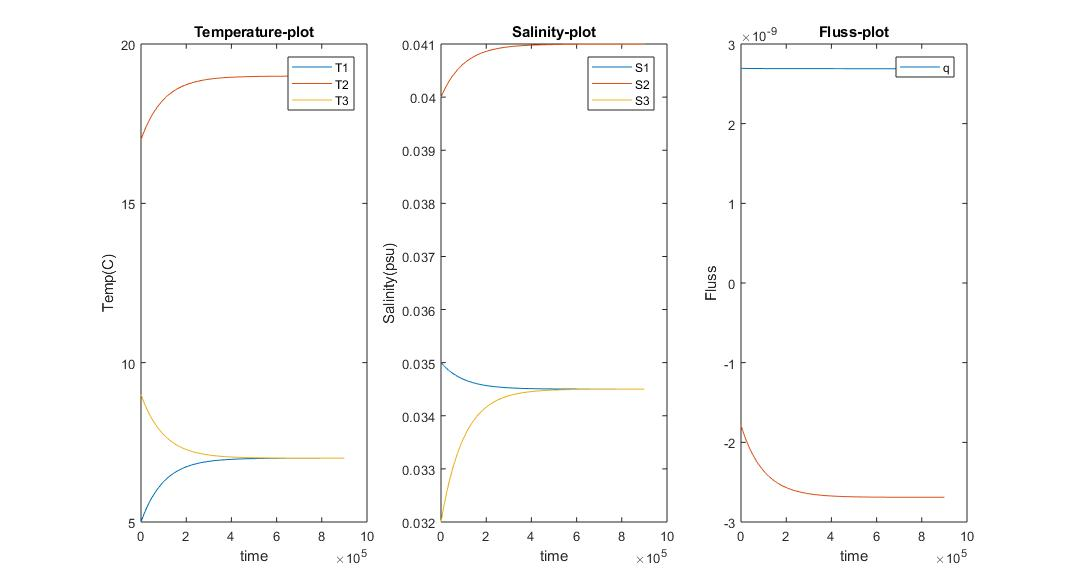
\includegraphics[width=14cm]{thermohalin/Code/graphs/result-3b2f-script.jpg}
	\centering
	\caption{Simulationsresultate}
	\label{thermohalin:simulationsresultate}
\end{figure}

Durch die Entkoppelung der zwei Flüsse, war es möglich, dass ein Fluss seine Richtung ändert.
Die Simulation hat zwar funktioniert, nur ist das Modell fehlerhaft. Wir müssen also unsere Darstellung des Modells anpassen. In der mittleren Box muss eine Absinkstelle eingefügt werden, damit das Modell mit der Simulation übereinstimmt. Das Resultat der Anpassung ist in Abbildung \ref{thermohalin:3b2f-inverted} zu sehen.

\begin{figure}
	\centering
	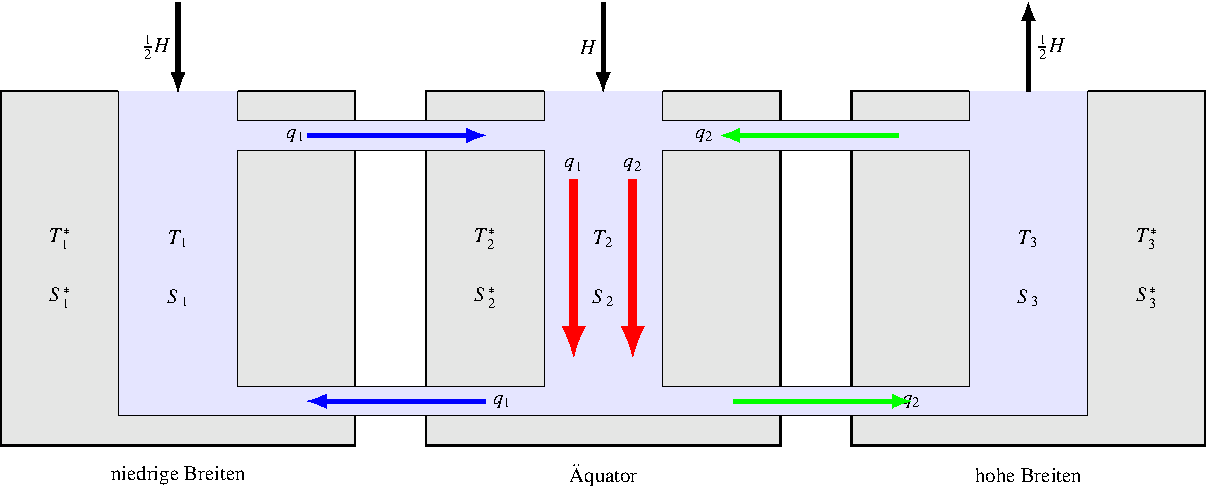
\includegraphics[width=14cm]{thermohalin/tikz/3b2f-inverted.pdf}
	\caption{Angepasstes Zwei-Fluss Modell}
	\label{thermohalin:3b2f-inverted}
\end{figure}

So lässt sich die entstandene Absinkstelle gut erkennen. 
Mit diesem Modell lässt sich der Golfstrom also nicht erfolgreich simulieren. 

\subsection{Ein-Fluss Modell (2. Ansatz)}\label{thermohalin:3b1f_title}

Dieses Modell ist der verbesserte Nachfolger des Zwei-Fluss Modelles.
Es stammt aus einer Aufgabe von {\em Mathematics and Climate}\cite{skript:kaperengler}.

Um zu verhindern, dass in der mittleren Box eine zusätzliche Absinkzone entsteht, muss dieser Weg versperrt werden. Das erreicht man am einfachsten, wenn der Tiefenstrom von der Äquatorbox getrennt wird. Die Äquatorzone ist nur via Oberflächenströmungen mit den anderen Boxen verbunden und die Tiefenströmung verbindet die Polzonen.


\begin{figure}
	\centering
	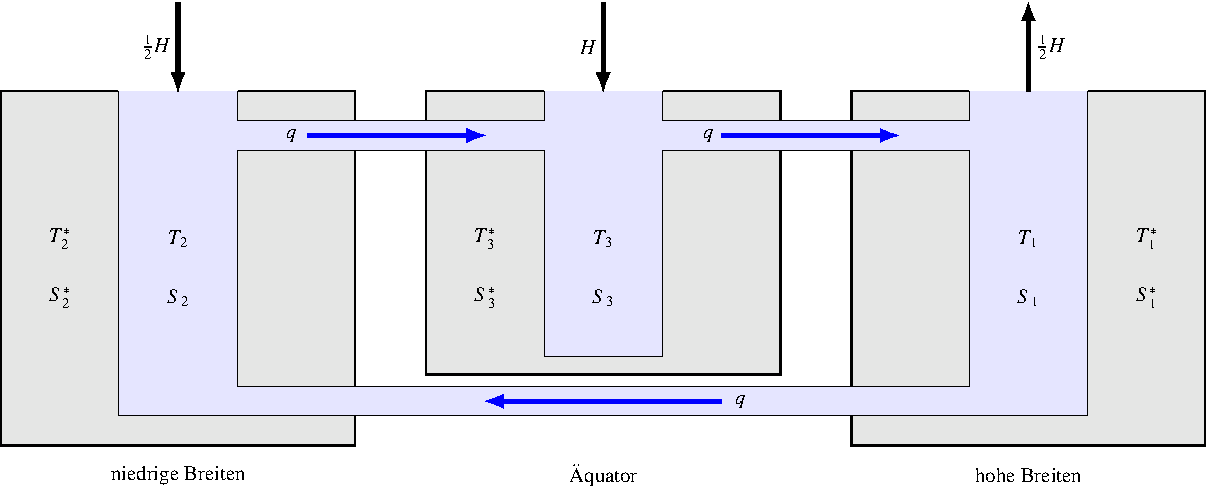
\includegraphics[width=14cm]{thermohalin/tikz/3b1f.pdf}
	\caption{Ein-Fluss Modell des THC}
	\label{thermohalin:3b1f}
\end{figure}

Wie im vorherigen Modell werden je drei Gleichungen für Temperatur- und Salinitätsänderung der jeweiligen Boxen benötigt.
Die einzelnen Boxen sind im Gegensatz zu 1. Versuch nur noch  mit einem Fluss verbunden. Das stimmt auch viel besser mit der Realität überein. Folgend ist die Gleichung für Box Nr. 1 dargestellt, um die Zusammenhänge zu erläutern:

\begin{equation}
\frac{dT_1}{dt} = c(T_p-T_1)+ \begin{cases} q(T_3-T_1)  \quad q>0 \\ |q|(T_2-T_1)  \quad q<0 \end{cases}
\end{equation}

Der erste Term beschreibt wie bisher den Temperaturaustausch zwischen Box und Reservoir und wurde in  Abschnitt \ref{thermohalin:3b2f_title} bereits erläutert. Der Flussterm ist jetzt anders, da der Fluss je nach Flussrichtung von anderen Boxen getrieben wird. Die Differenz muss jeweils zwischen der Quellbox und der betrachteten Box berechnet werden, da der Energie- und Salztransport jeweils nur vom Unterschied abhängt.
Wenn der Fluss positiv ist, also $q>0$, dann wird für die Berechnung Box 3 und die aktuelle Box verwendet, da die dritte Box die Quellbox darstellt. Wenn der Fluss nun negativ wird, ist die Quellbox Box 2 also muss hier die Differenz zwischen der zweiten und der dritten Box berechnet werden. Um die Simulation zu erleichtern, wird im Falle eines negativen Flusses mit dem Absolutbetrag gerechnet. Damit die Resultate trotzdem stimmen werden  bei der Differenzbildung jeweils die Terme vertauscht damit die Richtung trotzdem korrekt ist. 

Der Fluss $q$ wird ebenfalls anders berechnet, er ist nur vom Dichteunterschied zwischen den jeweiligen Polen abhängig \cite{skript:kaperengler}.
Wir können also wieder schreiben

\begin{equation}
q = k\frac{\varrho_1-\varrho_2}{\varrho_0}
\end{equation}

woraus folgt

\begin{equation}
q= k\frac{\varrho_0[1-\alpha(T_1-T_0)+\beta(S_1-S_0)]-\varrho_0[1-\alpha(T_2-T_0)+\beta(S_2-S_0)]}{\varrho_0}
\end{equation}

Das lässt sich kürzen, woraus sich folgende Gleichung für den Fluss ergibt:

\begin{equation}
q = k[\alpha(T_2-T_1)-\beta(S_2-S_1)] 
\end{equation}

Die Gleichungen für die anderen Boxen lassen sich nach dem gleichen Schema erstellen. Nur müssen jeweils entsprechend der Flussrichtung andere Quellboxen verwendet werden. Das gesamte Gleichungssystem hat dann folgende Form

\begin{equation}
\begin{aligned}
\frac{dT_1}{dt} &= c(T_p-T_1)&+ \begin{cases} q(T_3-T_1) & \quad q>0 \\ |q|(T_2-T_1) & \quad q<0 \end{cases}
\\
\frac{dT_2}{dt} &= c(T_p-T_2)&+\begin{cases} q(T_1-T_2) & \quad q>0 \\ |q|(T_3-T_2) & \quad q<0 \end{cases}
\\
\frac{dT_3}{dt} &= c(T_e-T_3)&+\begin{cases} q(T_2-T_3) & \quad q>0 \\ |q|(T_1-T_3) & \quad q<0 \end{cases}
\end{aligned}
\end{equation}
\begin{equation}
\begin{aligned}
\frac{dS_1}{dt} &= -H/2 &+ d(S_p-S_1)&+\begin{cases} q(S_3-S_1) & \quad q>0 \\ |q|(S_2-S_1) & \quad q<0 \end{cases}
\\
\frac{dS_2}{dt} &= \phantom{-}H &+ d(S_p-S_2)&+\begin{cases} q(S_1-S_2) & \quad q>0 \\ |q|(S_3-S_2) & \quad q<0 \end{cases}	
\\
\frac{dS_3}{dt} &= -H/2 &+d(S_e-S_3)&+\begin{cases} q(S_2-S_3) & \quad q>0 \\ |q|(S_1-S_3) & \quad q<0 \end{cases}
\end{aligned}
\end{equation}

\begin{equation}
q = k[\alpha\Delta T-\beta\Delta S].
\end{equation}



Aufgrund diese Gleichungen kann der neue Matlabcode geschrieben werden, welcher im nächsten Abschnitt erklärt wird.


\subsubsection{Matlab-code}

Die Übergabe der Startwerte und Konstanten, der Aufruf des Differentialgleichungslösers und das Plotten der Resultate sind identisch und werden deshalb nicht noch einmal gezeigt ( siehe  \ref{thermohalin:listing:input}). Nur die Funktion wurde verändert. Je nachdem ob der Fluss positiv oder negativ ist muss ein anderer Fall der Gleichungen berechnet werden. Dies wird mit einem \texttt{if}-Statement erreicht, welches in jedem Durchgang neu ausgewertet wird. 

\lstinputlisting[style=Matlab]{thermohalin/listings/listing-3b1f-solve.m}


\subsubsection{Resultate} 

Nach mehrfacher Simulation scheint es so, dass dieses Modell tatsächlich funktioniert. Für Werte, welche realen Werten entsprechen, reagiert die Simulation wie der richtige Golfstrom. Der Golfstrom fliesst vom Süd- zum Nordpol, sinkt dort ab und fliesst am Meeresgrund wieder bis zum Südpol, wo er aufsteigt und so den Kreislauf schliesst. Ein Plot der Resultate ist in Abbildung \ref{thermohalin:3b1f-skript} dargestellt.

Wie die Abbildung zeigt bleiben die Temperaturen ungefähr konstant. Dies liegt daran, dass die Temperaturstartwerte schon den Reservoirwerten angepasst wurden, was bedeutet dass diese Anpassung schon geschehen ist. Beim Salinitätsplot ist klar der Effekt des virtuellen Salzflusses zu sehen, welcher dazu führt, dass die Salinität in der Äquatorregion leicht steigt und in Polnähe dementsprechend abnimmt. Das Resultat stimmt und der Golfstrom fliesst in die uns bekannte Richtung.

\begin{figure}
	\centering
	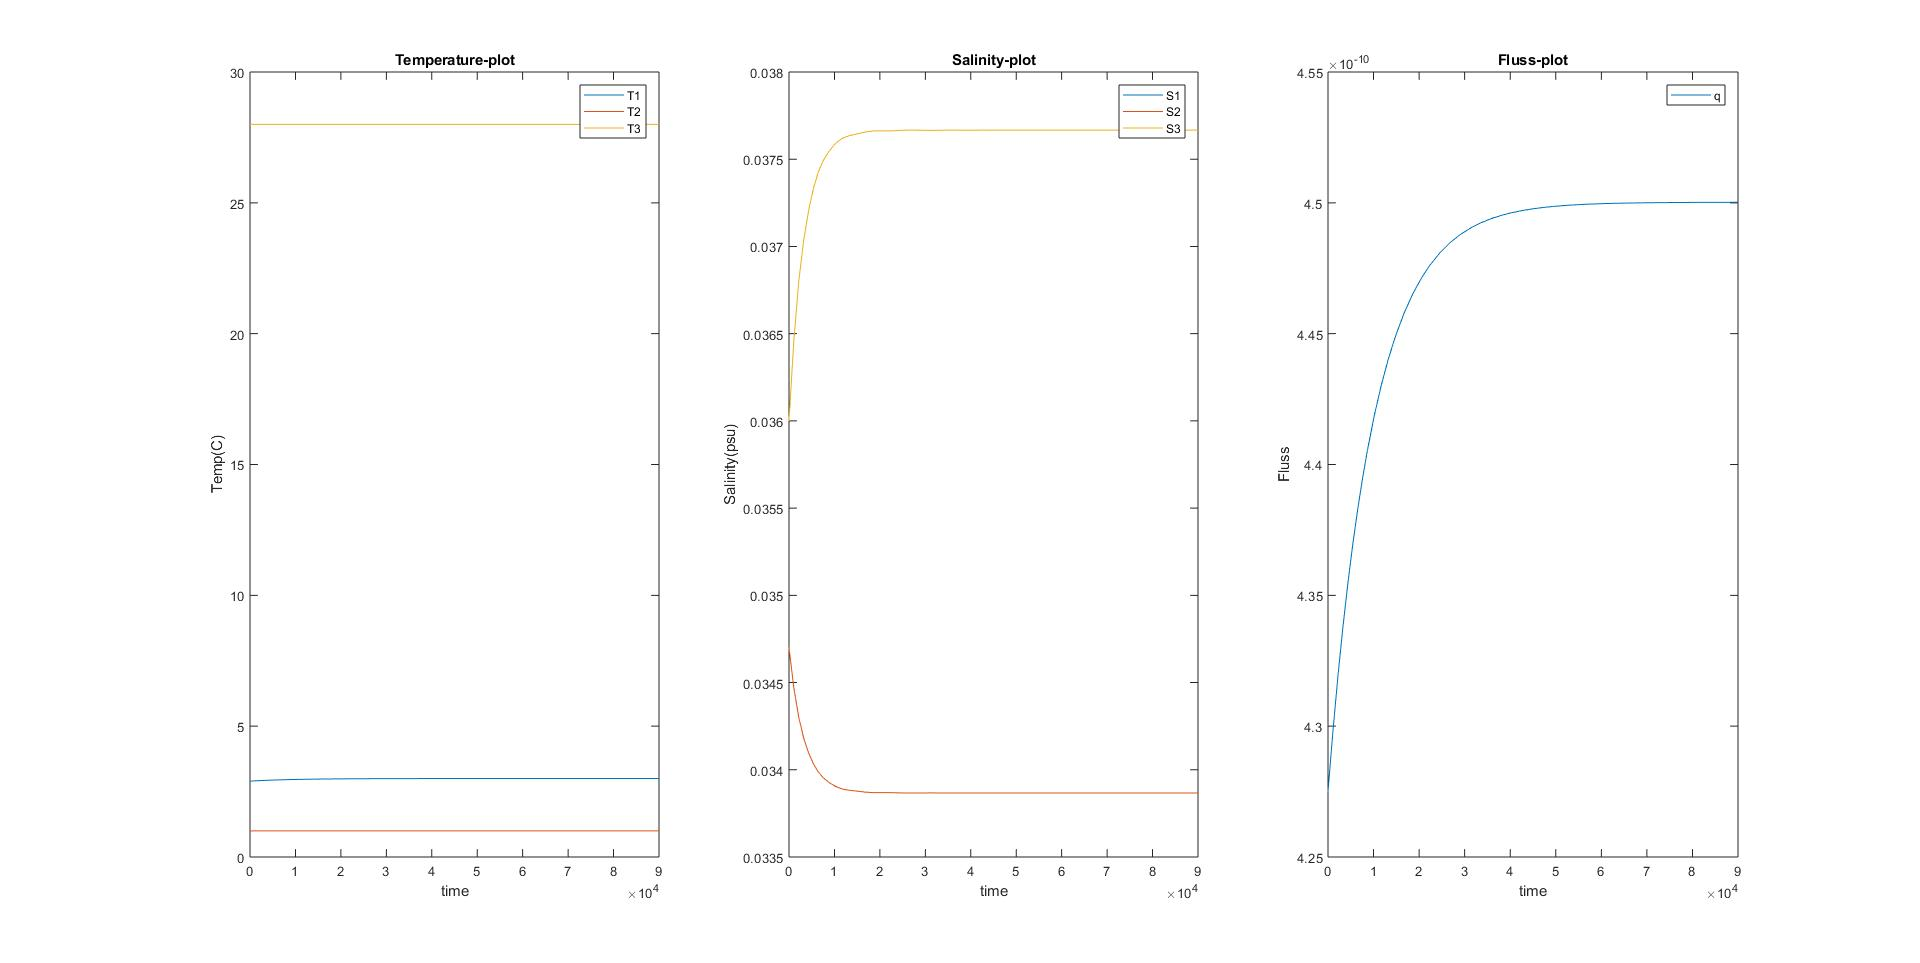
\includegraphics[width=14cm]{thermohalin/Code/graphs/3b1f-skript.jpg}
	\caption{Resultat der Ein-Fluss Simulation ohne Klimawandel}
	\label{thermohalin:3b1f-skript}
\end{figure}

Spannend wird es, wenn die Reservoirvariablen so angepasst werden, dass sie eine Klimaerwärmung und deren Folgen darstellen. Wie bereits in Abschnitt \ref{thermohalin:EinflussKlimawandel} erläutert, muss dazu die Salinität am Nordpol und die Temperatur am Äquator erhöht werden. Dies sollte dazu führen, dass der Golfstrom schwächer wird, anhält oder gar seine Richtung ändert. 
Der Eingabevektor, welcher die Temperaturen und Salinitäten der Reservoire enthält wird also angepasst.
Die Werte von $S_1^*$ ( Salinität Nordpol) und $T_3^*$ (Temperatur Äquator) werden erhöht.

\begin{equation*}
const = \begin{pmatrix}T_{1}^{*} \\ T_{2}^{*} \\ T_{3}^{*} \\ S_{1}^{*} \\ S_{2}^{*} \\ S_{3}^{*}\end{pmatrix}
\end{equation*}



Bei einer kleinen Veränderung wird der Strom nur schwächer, je grösser die Abweichungen jedoch sind desto stärker wird der Effekt.
Bis sich die Richtung des Stromes ändert.
Das Resultat entspricht also den Erwartungen. 

\begin{figure}
	\centering
	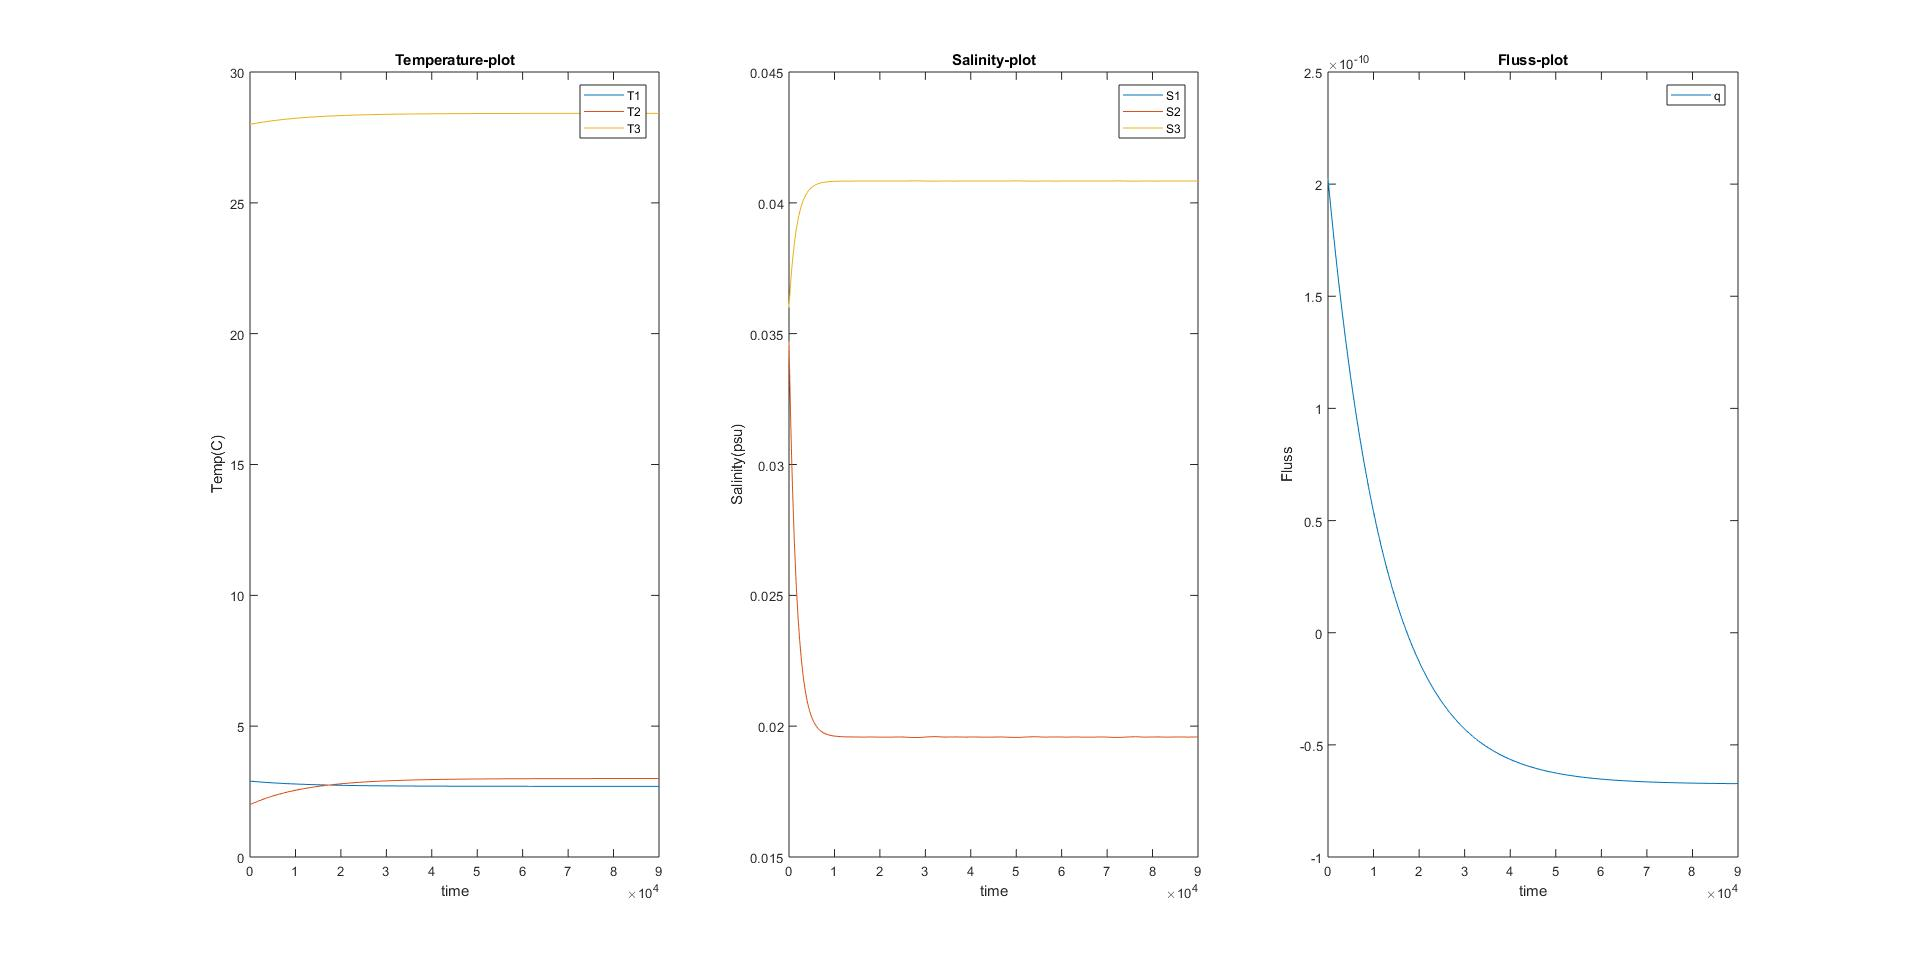
\includegraphics[width=14cm]{thermohalin/Code/graphs/3b1f-skript-klimawandel.jpg}
	\caption{Resultat der Ein-Fluss Simulation mit Klimawandel}
	\label{thermohalin:3b1f-skript-klimawandel}
\end{figure}

Wenn die Simulationsergebnisse mit dem Paper von Liu Wei \cite{thermohalin:liuwei} verglichen werden, lassen sich ähnliche Resultate feststellen.



	
	\section{Schlussfolgerung/Fazit}
\rhead{Schlussfolgerung/Fazit}

Es ist erstaunlich, wie sich die Realität mittels eines, auf den ersten Blick ziemlich simplen, Modelles nachstellen lässt. Trotzdem ist die Simulation mit Vorsicht zu geniessen, da die Resultate nur qualitativ zu interpretieren sind. Genaue Temperaturen und Salinitäten abzulesen ist in diesem Zustand der Simulation nicht möglich. Die Resultate sind eher als Trend in eine gewisse Richtung zu verstehen. Trotzdem ist es erfreulich, wie gut diese Simulation funktioniert. 
Als weiterer Schritt könnten noch die virtuellen Salzflüsse aufgeteilt werden um Nord- und Südpol unabhängig zu machen. Zusätzlich könnte die Simulation mit zuverlässigeren Daten füttern werden damit genauere Resultate entstehen. Auch sind die Zeitkonstanten der Salinität und Temperatur willkürlich gewählt, was aber keinen Einfluss auf die Simulation hat. Bei der genaueren Einstellung dieser Werte liesse sich vielleicht sogar eine Aussage über den Zeitraum machen. Dazu müsste aber das restliche Modell fehlerfrei sein, da diese Fehler wiederum die Resultate verfälschen würden.
Um tatsächlich Temperaturen und Salinitäten abzulesen müsste man die Simulation massiv erweitern, und grosse Datenmengen verwenden. Dies hätte jedoch den Rahmen dieses Projektes gesprengt. 
Die Forscher um Liu Wei \cite{thermohalin:liuwei} verwendeten die \texttt{NCAR SSCM3}\footnote{Die Software inklusive Dokumentation kann unter diesem Link bezogen werden: http://www.cesm.ucar.edu/models/ccsm4.0/} Simulation, welche dieser hier meilenweit überlegen ist. Diese Simulationssoftware ist in Module aufgeteilt, so lassen sich Wasser, Atmosphäre, Eis und Land separat oder in kombination simulieren. Das hat den grossen Vorteil, dass man bei der Strömungssimulation nicht nur den Ozean, sondern auch seine Wechselwirkung mit Atmosphäre und Kontinenten berücksichtigen kann. 
Schlussendlich war das Verstehen und Programmieren dieser Modelle sehr lehrreich. Der Einblick in das mathematische Gebiet der Simulation und deren Resultate waren sehr spannend. Schön ist auch, dass sich tatsächlich eine Simulation erstellen liess, welche, wenn auch nur rudimentär, tatsächlich die Realität wiedergibt.

Der gesamte Simulationscode welcher im Rahmen dieses Seminars erstellt wurde, ist im Unterkapitel \texttt{thermohalin} des Gitrepository des Seminarbuches abgelegt: texttt{https://github.com/AndreasFMueller/SeminarKlima}

	
	



\printbibliography[heading=subbibliography]
\end{refsection}